\documentclass[11pt,a4paper]{article}
\usepackage[margin=26mm]{geometry}
\usepackage[T1]{fontenc}
\usepackage{lmodern,microtype,amsmath,amssymb,amsthm,mathtools,mathrsfs}
\usepackage{booktabs,tabularx,array,xcolor,enumitem,graphicx,longtable}
\usepackage{fancyvrb,float}
\usepackage[colorlinks=true,linkcolor=blue!45!black,urlcolor=blue!45!black,citecolor=blue!45!black]{hyperref}
\hypersetup{pdftitle={Optimal entanglement witnesses under ellipsoid containment: the Milne-Jennings-Rudolph conjecture and its chirality correction},pdfauthor={Dev D. Goyal},pdfsubject={Two-qubit entanglement witnesses, steering ellipsoids, optimality within a set}}
\usepackage{fancyhdr}
\pagestyle{fancy}\fancyhf{}
\fancyhead[L]{\small Optimal witnesses under ellipsoid containment}
\fancyhead[R]{\small D. D. Goyal}
\fancyfoot[C]{\thepage}
\setlength{\headheight}{14pt}
\setlength{\parskip}{5pt}\setlength{\parindent}{0pt}
\newtheorem{theorem}{Theorem}
\newtheorem{lemma}[theorem]{Lemma}
\newtheorem{proposition}[theorem]{Proposition}
\newtheorem{corollary}[theorem]{Corollary}
\theoremstyle{definition}\newtheorem{definition}[theorem]{Definition}
\newcommand{\tr}{\operatorname{tr}}
\newcommand{\rank}{\operatorname{rank}}
\newcommand{\ran}{\operatorname{ran}}
\newcommand{\sgn}{\operatorname{sgn}}
\newcommand{\id}{\operatorname{id}}
\newcommand{\PSD}{\mathrm{PSD}}
\newcommand{\BP}{\mathrm{BP}}
\newcommand{\B}{\mathbb B^3}
\newcommand{\E}{\mathcal E}
\newcommand{\C}{\mathbb C}
\newcommand{\R}{\mathbb R}
\newcommand{\ket}[1]{\lvert #1\rangle}
\newcommand{\bra}[1]{\langle #1\rvert}
\newcommand{\proj}[1]{\ket{#1}\bra{#1}}
\newcommand{\XX}{X\otimes X}
\newcommand{\YY}{Y\otimes Y}
\newcommand{\ZZ}{Z\otimes Z}
\newcommand{\II}{I\otimes I}
\newcommand{\cstar}{c_*}
\newcommand{\Qstar}{Q_*}
\newcommand{\Sstar}{\mathcal S_*}
\theoremstyle{plain}\newtheorem*{theorem*}{Theorem}
\title{Optimal entanglement witnesses under ellipsoid containment:\\[2pt] the Milne--Jennings--Rudolph conjecture and its chirality correction}
\author{Dev D. Goyal}
\date{3 November 2026}
\begin{document}
\maketitle
\begin{abstract}
Milne, Jennings and Rudolph represented two-qubit entanglement witnesses by ellipsoids in the Bloch ball and conjectured, in Section~IV\,D of \emph{Geometric representation of two-qubit entanglement witnesses} (Phys.\ Rev.\ A \textbf{92}, 012311 (2015), arXiv:1407.8440): if $\E_*$ is an ellipsoid inside the Bloch sphere and $\Sstar$ is the set of witnesses whose ellipsoid lies inside $\E_*$, then the optimal witnesses in $\Sstar$ are represented by $\E_*$. We prove the conjecture as stated: every trace-one witness that is optimal in $\Sstar$ has ellipsoid exactly $\E_*$. The stronger reading, that every witness with ellipsoid $\E_*$ is optimal in $\Sstar$, is false. The witnesses $W_p$ of Example~2 of the same paper satisfy $W_p=\frac{p}{1-p}W_{1-p}+\frac{1-2p}{1-p}P_+$ with $P_+\succeq0$, so for every $0<p<1/2$ the left-handed witness $W_p$ and the right-handed witness $W_{1-p}$ have the same full-dimensional Class~D ellipsoid while $W_{1-p}$ detects strictly more states. The correct characterization needs chirality: for a full-dimensional admissible target the optimal witnesses are exactly the right-handed witnesses with ellipsoid $\E_*$; for a planar target they are exactly the witnesses with ellipsoid $\E_*$; segments and points represent no witness. Thus the unrestricted equivalence holds in Class~C and for planar targets and fails for full-dimensional Class~D targets. The proof uses the two-qubit decomposability theorem and the Avron--Kenneth Lorentz normal forms. We also give an exact $4\times4$ semidefinite containment test that covers singular targets, a polynomial optimality test, a convex program with a unique rank-one optimizer, and several order-theoretic and geometric consequences. A Lean~4 development checks the counterexample for actual complex $4\times4$ matrices against all complex density matrices, for the rational pair $p=1/4,3/4$ and for every $0<p<1/2$, together with further algebraic and geometric ingredients; the general classification is a conventional proof, and its Lean assembly is stated with its structural hypotheses explicit.
\end{abstract}
\clearpage
\setcounter{tocdepth}{1}
\begingroup
\small
\setlength{\parskip}{0pt}
\tableofcontents
\endgroup
\clearpage

\section{Introduction}

\paragraph{The question in plain terms.} An entanglement witness is an observable whose expectation value is negative on some entangled states and nonnegative on every separable state; one witness is \emph{finer} than another if it detects every state the other detects. For two qubits, Milne, Jennings and Rudolph drew each witness as an ellipsoid inside the Bloch ball, together with a handedness (chirality) sign. They asked: if we only allow witnesses whose ellipsoid fits inside a fixed ellipsoid $\E^\star$, are the best (optimal) ones exactly those that fill $\E^\star$? \emph{Answer:} every optimal witness does fill $\E^\star$, so their conjecture as printed is true; but filling $\E^\star$ is not enough, because a left-handed witness that fills a full-dimensional target can always be improved by a right-handed one with the same ellipsoid. The ellipsoid forgets exactly the information, chirality, that decides optimality.

Milne, Jennings and Rudolph \cite{milne} extended the quantum steering ellipsoid formalism from two-qubit states to arbitrary two-qubit block-positive operators. A unit-trace entanglement witness $W$ is then represented by an ellipsoid $\E(W)$ inside the Bloch ball, with a chirality sign, and optimality and weak optimality of $W$ become visible in $\E(W)$ \cite[Theorem~4]{milne}. Motivated by two examples (the set of all witnesses, whose optimal members fill the whole Bloch ball, and the set $EW_4$, whose optimal members fill the $xz$ unit disc), they stated the following conjecture in Section~IV\,D of \cite{milne}; we quote it verbatim from arXiv:1407.8440v2.

\begin{quote}
\textbf{Conjecture.} Let $\E^\star$ be an ellipsoid lying inside the Bloch sphere and $S$ be a set of two-qubit entanglement witnesses defined as follows: $W\in S$ if and only if $\E$ representing $W$ lies inside $\E^\star$. The optimal $W\in S$ are then represented by $\E=\E^\star$.
\end{quote}

The authors add that the conjecture applies to any $\E^\star$ belonging to Class~C or Class~D, and that it is nontrivial to approach analytically, partly because deciding whether one ellipsoid lies inside another is itself difficult. Here a witness $W\in S$ is optimal in $S$ if no member of $S$ is strictly finer, that is, detects a strictly larger set of states \cite{milne,lewenstein}. The conjecture is restated in Milne's doctoral thesis \cite{thesis}.

The printed sentence admits two readings. The \emph{necessity} reading says that every optimal $W\in S$ has $\E(W)=\E^\star$. The \emph{characterization} reading adds the converse, that the optimal members of $S$ are exactly the witnesses represented by $\E^\star$. The two motivating examples are consistent with both, because in them every witness filling the target is optimal. We show that the two readings have different answers.

\begin{theorem*}[Summary of the main results]
Let $\E_*$ be an ellipsoid in the Bloch ball that represents at least one witness, and let $\Sstar$ be the set of trace-one witnesses $W$ with $\E(W)\subseteq\E_*$.
\begin{enumerate}[label=(\alph*)]
\item \emph{(The conjecture holds.)} Every witness optimal in $\Sstar$ has $\E(W)=\E_*$; moreover every member of $\Sstar$ has a finer or equal member of $\Sstar$ whose ellipsoid is $\E_*$.
\item \emph{(The converse fails.)} For every $0<p<1/2$, the witnesses $W_p$ and $W_{1-p}$ of \cite[Example~2]{milne} have the same full-dimensional Class~D ellipsoid, and $W_{1-p}$ is strictly finer than $W_p$. Hence $W_p$ represents $\E_*=\E(W_p)$ but is not optimal in $\Sstar$.
\item \emph{(Corrected characterization.)} If $\E_*$ is full-dimensional, $W$ is optimal in $\Sstar$ if and only if $\E(W)=\E_*$ and $W$ is right-handed. If $\E_*$ is planar, $W$ is optimal in $\Sstar$ if and only if $\E(W)=\E_*$. Segments and points represent no witness.
\end{enumerate}
\end{theorem*}

Theorem~\ref{thm:main} below is the precise statement. In Class~C every witness filling a full-dimensional target is automatically right-handed, so the characterization reading is true there and for planar targets; it fails exactly for left-handed representatives of full-dimensional Class~D targets, which are always strictly improvable (Lemma~\ref{lem:mirror}). This is consistent with Theorem~4 of \cite{milne}, where optimality among all witnesses requires the whole Bloch ball \emph{and} right-handedness.

\paragraph{What is new and what is not.} The witness family $W_p$ is Example~2 of \cite{milne}, introduced earlier in the literature cited there; only its use to separate the two readings is new here. Positive-remainder subtraction and the fineness criterion are due to Lewenstein, Kraus, Cirac and Horodecki \cite{lewenstein}; best separable approximations and product-vector subtraction to Lewenstein--Sanpera and Karnas--Lewenstein \cite{ls,karnas}; best positive-part witness decompositions to Bru\ss{} et al.\ \cite{bruss}; semidefinite programming for optimal decompositions to Thiang--Raynal--Englert \cite{thiang}. The two external theorems on which the classification rests are the two-qubit decomposability theorem \cite{woronowicz} and the complete Lorentz normal forms of Avron and Kenneth \cite{avron}. The candidate contributions are the proof of the conjecture, the chirality correction for arbitrary admissible targets including singular and translated ones, and the consequences in Part~II. A bounded literature search through 3 November 2026, including the works citing \cite{milne}, found no earlier resolution of the conjecture; this is not a priority guarantee.

\paragraph{Verification scope.} A Lean~4 development (Lean 4.19.0, Mathlib \texttt{c44e0c8}) proves, for genuine complex $4\times4$ matrices, with states ranging over all complex density matrices and block positivity over all complex product vectors, the counterexample of part~(b) for the rational pair $p=1/4,3/4$ and for every $0<p<1/2$, its nonoptimality in every surrounding set containing the finer witness, and further ingredients listed in Appendix~\ref{app:formal}. Parts~(a) and~(c) are conventional proofs; their Lean assembly theorem takes the cofinality, incomparability and faithfulness inputs as explicit hypotheses. Exact SymPy scripts check the remaining finite identities and certificates. Appendix~\ref{app:formal} states the split precisely.

\paragraph{How the proof works.} The argument has four steps, each proved in Part~I.
\begin{enumerate}[label=\arabic*.]
\item \emph{Fineness is subtraction.} A normalized witness $V$ is finer than $W$ exactly when $W=\alpha V+P$ with $0<\alpha\le1$ and $P\succeq0$ (Lemma~\ref{lem:fine}). So improving a witness means peeling off a positive operator.
\item \emph{Pull back to the whole Bloch ball.} The target ellipsoid is the image of the Bloch ball under a positive qubit map $L$ (Section~\ref{sec:lift}). Every witness inside the target lifts through $L$ to a block-positive operator; decomposability and product-vector subtraction then refine it to the image of a single partially transposed entangled pure state, whose ellipsoid is the whole target. This gives necessity: an optimal witness must fill the target.
\item \emph{Chirality decides.} A left-handed representative of a full-dimensional target is strictly dominated by the right-handed one with the same ellipsoid (Lemma~\ref{lem:mirror}, using the Avron--Kenneth normal forms); this is where the converse fails, and $W_p$ versus $W_{1-p}$ is the simplest instance.
\item \emph{No improvement within one orbit.} Two witnesses with the same ellipsoid and the same chirality differ by a local filter on Bob's side, and such filters can never produce a strictly finer witness (Lemma~\ref{lem:orbit}, Corollary~\ref{cor:sameE}). This gives sufficiency of the corrected condition.
\end{enumerate}
Part~I contains the classification and the counterexample, Part~II further results (exact orders of the family $W_p$, a convex program with a unique optimizer, robustness, Class~C examples and decision rules), Section~\ref{sec:related} related work, and the appendices the formal verification scope and reproduction details.

\part{The conjecture and its analytic resolution}

\section{Main theorem and conventions}


We interpret ellipsoid containment as containment of the filled geometric sets; it does not impose a chirality constraint. This is the set definition in Section~IV\,D of \cite{milne}. Write
\[
 \E_*=\cstar+A\B,\qquad \Qstar=AA^{\mathsf T},\qquad \B=\{u\in\R^3:\|u\|\leq1\}.
\]
An admissible target here means that at least one witness is represented by that ellipsoid. All operators below are on $\C^2\otimes\C^2$, unless otherwise stated. Partial transpose on Bob is denoted $\Gamma$.

\begin{theorem}[Complete classification]\label{thm:main}
Let $\E_*\subseteq\B$ be admissible, and define
\[
 \Sstar=\{W:\ W\text{ is a trace-one entanglement witness},\ \E(W)\subseteq\E_*\}.
\]
Then every $W\in\Sstar$ has a finer or equal witness $U\in\Sstar$ with $\E(U)=\E_*$. Moreover:
\begin{enumerate}[label=(\roman*)]
\item If $\rank\Qstar=3$, $W$ is optimal in $\Sstar$ if and only if $\E(W)=\E_*$ and $\chi(W)=+1$.
\item If $\rank\Qstar=2$, $W$ is optimal in $\Sstar$ if and only if $\E(W)=\E_*$. These witnesses have $\chi(W)=0$.
\item If $\rank\Qstar\leq1$, the containment set contains no witnesses, so such a target is not admissible.
\end{enumerate}
In particular, the literal necessary implication in the paper is valid in both Classes C and D. Its unrestricted converse fails in full-dimensional Class D.
\end{theorem}

\begin{center}
\begin{tabularx}{\linewidth}{@{}l l X@{}}
\toprule
Target & Dimension & Optimal witnesses in the containment set\\
\midrule
Class C & 3 & Exactly the witnesses with $\E(W)=\E_*$; their chirality is necessarily $+1$.\\
Class D & 3 & Exactly the witnesses with $\E(W)=\E_*$ and chirality $+1$. Left-handed representatives are strictly improvable.\\
Class D & 2 & Exactly the witnesses with $\E(W)=\E_*$.\\
Line or point & 0 or 1 & No witnesses.\\
\bottomrule
\end{tabularx}
\end{center}

The proof is a complete mathematical argument using named published inputs. Those inputs are not new claims of this work. The exact counterexample and its detection relation are machine checked separately. The expanded formal development and its remaining gaps are documented in Appendix~\ref{app:formal}. No claim of an end-to-end Lean formalization of Theorem~\ref{thm:main}, or of established publication priority, is made.

\section{Definitions and matrix conventions}

A Hermitian operator $W$ is block positive if
\[
 \bra{x\otimes y}W\ket{x\otimes y}\geq0\quad\text{for every }x,y\in\C^2.
\]
It is an entanglement witness if it is block positive but not positive semidefinite. We normalize witnesses by $\tr W=1$. Its detected states are
\[
 D(W)=\{\rho\succeq0:\tr\rho=1,\ \tr(\rho W)<0\}.
\]
The witness $V$ is finer than $W$ when $D(W)\subseteq D(V)$; strict fineness means proper inclusion. Optimality in a specified set excludes a distinct strictly finer member of that set.

Using the standard Pauli matrices $X,Y,Z$, write
\begin{equation}\label{eq:bloch}
 W=\frac14\left(\II+a\cdot\sigma\otimes I+I\otimes b\cdot\sigma+
       \sum_{i,j=1}^3 T_{ij}\sigma_i\otimes\sigma_j\right),
 \qquad \Theta_W=\begin{pmatrix}1&b^{\mathsf T}\\a&T\end{pmatrix}.
\end{equation}
For a Bob effect with Bloch vector $u\in\B$, the normalized conditional Alice vector is
\begin{equation}\label{eq:fractional}
 r_W(u)=\frac{a+Tu}{1+b\cdot u}.
\end{equation}
Its range is the filled ellipsoid $\E(W)$. The denominator is strictly positive for witnesses, by the next lemma.

\begin{lemma}[A witness has a nonsingular Bob marginal]\label{lem:marginal}
If $W$ is a two-qubit witness, then $W_B=\tr_A W\succ0$; equivalently, $\|b\|<1$.
\end{lemma}
\begin{proof}
Block positivity makes $W_B$ positive semidefinite. If it has a kernel vector, choose a Bob basis in which that vector is first. The corresponding Alice diagonal block of $W$ is positive semidefinite with zero trace, hence zero. Write the other blocks as
\[
 W=\begin{pmatrix}0&C\\C^\dagger&D\end{pmatrix}_{\!B}.
\]
For every Alice vector $x$, the $2\times2$ matrix of Bob expectations in $x$ is positive semidefinite. Its zero first diagonal entry forces $x^\dagger Cx=0$. Complex polarization gives $C=0$. Block positivity also gives $D\succeq0$, so $W\succeq0$, a contradiction.
\end{proof}

Whitening Bob gives the canonical witness
\[
 \widetilde W=(I\otimes(2W_B)^{-1/2})W(I\otimes(2W_B)^{-1/2})
 =\frac14\left(\II+c\cdot\sigma\otimes I+
 \sum_{i,j}\widetilde T_{ij}\sigma_i\otimes\sigma_j\right).
\]
Its ellipsoid is $c+\widetilde T\B$, with $Q=\widetilde T\widetilde T^{\mathsf T}$ and $\chi=\sgn\det\widetilde T$. In terms of the original data, set $\gamma^2=(1-\|b\|^2)^{-1}$; then
\begin{align}
 c&=\gamma^2(a-Tb),\\
 Q&=\gamma^2(T-ab^{\mathsf T})(I+\gamma^2bb^{\mathsf T})(T^{\mathsf T}-ba^{\mathsf T}).\label{eq:shape}
\end{align}
The chirality sign can also be computed as $\sgn\det\Theta_W$, since whitening has positive determinant on the real Pauli coefficient space.

For a block-positive two-qubit operator, Class C means $W\not\succeq0$ but $W^\Gamma\succeq0$, and Class D means both $W$ and $W^\Gamma$ fail to be positive semidefinite. The determinant characterization in \cite{milne} gives the corresponding strict signs for witnesses. The proof below uses positivity itself, so it does not rely on determinants near a numerical threshold.

\section{Exact containment and fineness inequalities}

\subsection{Canonical containment, including a singular target}

Let $H=\Qstar^+$ be the Moore--Penrose inverse, let $\Pi=\Qstar\Qstar^+$ be the orthogonal support projector, and let $d=c-\cstar$. Then
\begin{equation}\label{eq:contain-support}
 (I-\Pi)d=0,\qquad (I-\Pi)\widetilde T=0
\end{equation}
are necessary support conditions. Subject to these conditions,
\begin{equation}\label{eq:contain-lmi}
 \E(W)\subseteq\E_*
 \quad\Longleftrightarrow\quad
 \exists\lambda\geq0:\
 \begin{pmatrix}
 \lambda I_3-\widetilde T^{\mathsf T}H\widetilde T&-\widetilde T^{\mathsf T}Hd\\
 -d^{\mathsf T}H\widetilde T&1-d^{\mathsf T}Hd-\lambda
 \end{pmatrix}\succeq0.
\end{equation}
Indeed, membership in the outer ellipsoid is equivalent to support membership and $(x-\cstar)^{\mathsf T}H(x-\cstar)\leq1$. Substitute $x=c+\widetilde T u$. The S-lemma \cite{polik} applies with the strictly feasible ball constraint $1-\|u\|^2\geq0$ (take $u=0$), and gives precisely \eqref{eq:contain-lmi}. The support constraints are essential for a flat target; merely replacing an inverse by a pseudoinverse would be incorrect.

\subsection{An equivalent criterion before whitening}

Define
\[
 h=a-\cstar,\qquad D=T-\cstar b^{\mathsf T}.
\]
The support conditions are $(I-\Pi)h=0$ and $(I-\Pi)D=0$. Because $1+b\cdot u>0$, containment is equivalent to
\[
 (1+b\cdot u)^2-(h+Du)^{\mathsf T}H(h+Du)\geq0
 \qquad(\|u\|\leq1).
\]
Consequently its exact matrix certificate is
\begin{equation}\label{eq:raw-lmi}
 \exists\lambda\geq0:\quad
 \begin{pmatrix}
 \lambda I_3+bb^{\mathsf T}-D^{\mathsf T}HD&b-D^{\mathsf T}Hh\\
 b^{\mathsf T}-h^{\mathsf T}HD&1-h^{\mathsf T}Hh-\lambda
 \end{pmatrix}\succeq0.
\end{equation}
This is an exact test for fixed Bloch data. Its entries are quadratic in those data; it is not being asserted to be jointly affine in all unknown entries of $W$.

\subsection{Fineness is positive semidefinite subtraction}

\begin{lemma}[Fineness criterion]\label{lem:fine}
For trace-one witnesses $W,V$,
\begin{equation}\label{eq:fine}
 D(W)\subseteq D(V)
 \quad\Longleftrightarrow\quad
 W=\alpha V+P,\qquad 0<\alpha\leq1,\quad P\succeq0.
\end{equation}
Strict inclusion is equivalent to $P\neq0$, and then $\alpha<1$. Equivalently, there exists $t\geq1$ with $tW-V\succeq0$.
\end{lemma}
\begin{proof}
The reverse implication follows by taking expectations. For the forward implication, contraposition gives $\tr(V\rho)\geq0\Rightarrow\tr(W\rho)\geq0$ for every $\rho\succeq0$. The dual cone of $\{\rho\succeq0:\tr(V\rho)\geq0\}$ is $\PSD+\R_+V$. This sum is closed: if a convergent sequence $P_n+\alpha_nV$ had unbounded $\alpha_n\geq0$, division by $\alpha_n$ would give $-V\succeq0$, impossible for a trace-one witness. Thus $W=P+\alpha V$. Since $W$ is not positive semidefinite, $\alpha>0$; taking traces gives $\alpha\leq1$.

If inclusion held in both directions, there would also be $V=\beta W+Q$ with $0<\beta\leq1$ and $Q\succeq0$. Substitution gives $(1-\alpha\beta)W=P+\alpha Q\succeq0$. As $W$ is a witness, $\alpha\beta=1$ and consequently $\alpha=\beta=1$, $P=Q=0$. Hence normalized witnesses with the same detection set are equal. This proves the strictness assertion. The criterion is also the standard witness refinement relation of \cite{lewenstein}.
\end{proof}

Together, \eqref{eq:contain-support}--\eqref{eq:contain-lmi} and \eqref{eq:fine} translate the original optimization problem into exact matrix conditions. Theorem~\ref{thm:main} goes further: it eliminates the search for an improving witness.

\subsection{Optimality without any remaining optimization}

For an already certified witness and admissible target, put
\[
 \delta=1-\|b\|^2>0,\qquad K=T-ab^{\mathsf T}.
\]
Theorem~\ref{thm:main} and \eqref{eq:shape} give the following exact algebraic test:
\begin{equation}\label{eq:polynomial-optimality}
 \boxed{\begin{aligned}
 a-Tb&=\delta\cstar,\\
 K(\delta I_3+bb^{\mathsf T})K^{\mathsf T}&=\delta^2\Qstar,\\
 \det K&\geq0.
 \end{aligned}}
\end{equation}
These conditions are equivalent to relative optimality. The determinant is strictly positive in rank three and zero in rank two. They are polynomial equalities and an inequality in the original Bloch data; no canonical square root, semidefinite optimization, or filter search remains.

\begin{corollary}[The test also certifies witness validity]\label{cor:algebraic-validity}
Let $W$ be any trace-one Hermitian operator, and let $\E_*$ be an admissible target. Then $W$ is a witness optimal in $\Sstar$ if and only if $\delta>0$ and all three conditions in \eqref{eq:polynomial-optimality} hold.
\end{corollary}
\begin{proof}
Necessity follows from Theorem~\ref{thm:main}. Conversely, $\delta>0$ makes every steering denominator positive. The first two equations and the exact shape formula give $\E(W)=\E_*\subseteq\B$, so every conditional Alice operator is positive; hence $W$ is block positive. The determinant condition gives positive chirality in rank three and zero in rank two. Choose a known witness for the admissible target and, in rank three, use the mirror lemma if necessary to choose positive chirality. The same-ellipsoid, same-chirality filter correspondence in Corollary~\ref{cor:sameE} relates it to $W$ by an invertible Bob congruence and positive normalization. Failure of positive semidefiniteness is preserved. Thus $W$ is a witness, and the classification proves its relative optimality.
\end{proof}

The strict marginal inequality cannot be dropped. For any product state with a pure Bob factor, $\|b\|=1$ and $T=ab^{\mathsf T}$. Thus $\delta=0$, $K=0$, and $a-Tb=0$. All three displayed polynomial conditions then hold for \emph{every} target, although the operator is positive semidefinite and is not a witness. Trace normalization, Hermiticity, target admissibility and $\delta>0$ are essential domain conditions of the strengthened test.

For a full-dimensional target the equations simplify further. Put $D=T-\cstar b^{\mathsf T}$. Under the same domain conditions, relative optimality is equivalent to
\begin{equation}\label{eq:quadratic-optimality}
 \boxed{a-Tb=\delta\cstar,\qquad
 D^{\mathsf T}\Qstar^{-1}D=\delta I_3+bb^{\mathsf T},\qquad
 \det D>0.}
\end{equation}
The matrix equalities are quadratic in the original Bloch coefficients, with the target fixed. To verify equivalence, the centre equation gives $a-\cstar=Db$ and hence $K=D(I-bb^{\mathsf T})$. Since
\[
 (I-bb^{\mathsf T})(\delta I+bb^{\mathsf T})=\delta I,
\]
the shape equation is $D(I-bb^{\mathsf T})D^{\mathsf T}=\delta\Qstar$. Invertibility gives the displayed inverse-metric equation, and $\det K=\delta\det D$ gives the orientation sign. This reformulation applies only to a nonsingular target; the polynomial criterion above covers planar targets without using an inverse.

\section{An exact counterexample to the unrestricted converse}

For $0\leq p\leq1$, define
\begin{equation}\label{eq:Wp}
 W_p=\frac12\begin{pmatrix}
 p&0&0&0\\0&1-p&1&0\\0&1&1-p&0\\0&0&0&p
 \end{pmatrix}.
\end{equation}
This family already occurs in Example 2 of \cite{milne}; the comparison below is an immediate exact consequence, not a claim that the family itself is new. Let
\[
 \ket{\psi^\pm}=\frac{\ket{01}\pm\ket{10}}{\sqrt2},\qquad
 P_+=\proj{\psi^+},\qquad F\ket{x,y}=\ket{y,x}.
\]
Then $W_p=pF/2+(1-p)P_+$. Both summands are block positive, since the product expectation of $F$ is $|\langle x,y\rangle|^2$. Also
\[
 \operatorname{spec}(W_p)=\left\{\frac p2,\frac p2,\frac{2-p}{2},-\frac p2\right\}.
\]
Thus every $0<p\leq1$ is a witness. For $0<p<1$,
\begin{equation}\label{eq:dets}
 \det W_p=-\frac{p^3(2-p)}{16}<0,
 \qquad \det W_p^\Gamma=-\frac{(1-p)^3(1+p)}{16}<0,
\end{equation}
so these are Class D.

Take $W=W_{1/4}$ and $V=W_{3/4}$. Explicitly,
\[
 W=\frac18\begin{pmatrix}1&0&0&0\\0&3&4&0\\0&4&3&0\\0&0&0&1\end{pmatrix},
 \qquad
 V=\frac18\begin{pmatrix}3&0&0&0\\0&1&4&0\\0&4&1&0\\0&0&0&3\end{pmatrix}.
\]
Their canonical correlation matrices are $\operatorname{diag}(1,1,-1/2)$ and $\operatorname{diag}(1,1,1/2)$. They have exactly the same ellipsoid
\begin{equation}\label{eq:exampleE}
 \E_* = \{(x,y,z):x^2+y^2+4z^2\leq1\}\subseteq\B,
\end{equation}
but opposite chiralities. The exact identity
\begin{equation}\label{eq:counter-id}
 \boxed{W=\frac13 V+\frac23P_+}
\end{equation}
proves $D(W)\subsetneq D(V)$. Strictness can also be seen without invoking Lemma~\ref{lem:fine}: the density matrix
\[
 \rho=\tfrac34\proj{\psi^-}+\tfrac14\proj{\psi^+}
 =\begin{pmatrix}0&0&0&0\\0&1/2&-1/4&0\\0&-1/4&1/2&0\\0&0&0&0\end{pmatrix}
\]
satisfies
\[
 \tr(\rho W)=\frac18>0,\qquad \tr(\rho V)=-\frac18<0.
\]
The determinant pairs are $(-7/4096,-135/4096)$ for $W$ and $(-135/4096,-7/4096)$ for $V$, where each pair lists the operator and its partial transpose.

There is also an improvement that preserves negative chirality. Set $V'=W_{1/3}$. Then
\[
 W=\frac34V'+\frac14P_+,
 \qquad
 \E(V')=\{x^2+y^2+9z^2\leq1\}\subsetneq\E_*.
\]
Both $W$ and $V'$ are left-handed Class D witnesses. Therefore the simple claim that filling a given ellipsoid guarantees optimality fails even if the improving witness is required to have the same chirality. For example $\rho'=\tfrac67\proj{\psi^-}+\tfrac17\proj{\psi^+}$ gives $\tr(\rho'W)=1/56$ and $\tr(\rho'V')=-1/42$.

\subsection{The failure also occurs strictly inside the Bloch ball}

It is not a consequence of contact with the Bloch sphere. Set
\[
 H_\pm=\frac14\left(\II+\frac34\XX+\frac34\YY\pm\frac14\ZZ\right).
\]
Both are Class D, have semiaxes $(3/4,3/4,1/4)$, and have expectation at least $1/16$ on every normalized product vector. Their Bell spectra are $(5,5,9,-3)/16$ and $(3,3,11,-1)/16$, respectively. With $\ket{\phi^\pm}=(\ket{00}\pm\ket{11})/\sqrt2$,
\[
 H_-=\tfrac13H_++\tfrac1{12}\proj{\phi^+}+\tfrac1{12}\proj{\phi^-}+\tfrac12\proj{\psi^+}.
\]
This is another exact positive-remainder certificate. The state $\tfrac45\proj{\psi^-}+\tfrac15\proj{\psi^+}$ gives expectations $7/80$ for $H_-$ and $-3/80$ for $H_+$. These additional identities are verified by the exact symbolic scripts of the package.

\section{Incomparability inside a Bob-filter orbit}

\begin{lemma}[One-sided filters cannot give strict fineness within an orbit]\label{lem:orbit}
Let $W$ be block positive but not positive semidefinite on $\C^m\otimes\C^2$, with positive definite Bob marginal. If
\[
 P=W-(I\otimes G)W(I\otimes G^\dagger)\succeq0,
\]
then $P=0$.
\end{lemma}
\begin{proof}
Apply a common Bob whitening congruence and rescale so that $W_B=I/2$. The transformed identity has the same form, with a possibly different $G$. Taking the Alice partial trace gives $I-GG^\dagger\succeq0$; hence $G$ is a contraction.

If its spectral radius is less than one, iterate the identity:
\[
 W=\sum_{j=0}^{n-1}(I\otimes G^j)P(I\otimes(G^\dagger)^j)
 +(I\otimes G^n)W(I\otimes(G^\dagger)^n).
\]
The final term tends to zero. Every summand is positive semidefinite, so closedness of the positive semidefinite cone implies $W\succeq0$, a contradiction.

Otherwise $G$ has an eigenvalue $\lambda$ of modulus one. Its eigenvector is reducing: equality in the contraction inequality yields $G^\dagger v=\bar\lambda v$. As Bob has dimension two, a unitary change of basis gives $G=\operatorname{diag}(\lambda,\mu)$ with $|\mu|\leq1$. If $|\mu|=1$, $G$ is unitary and $\tr P=0$, so $P=0$.

If $|\mu|<1$, write the Bob blocks of $W$ as $\bigl(\begin{smallmatrix}A&C\\C^\dagger&D\end{smallmatrix}\bigr)$. Block positivity implies $A,D\succeq0$. The first diagonal block of $P$ is zero, so positivity of $P$ forces its off-diagonal block $(1-\lambda\bar\mu)C$ to vanish. This coefficient is nonzero; thus $C=0$, again making $W$ positive semidefinite. This contradiction exhausts the cases.
\end{proof}

\begin{corollary}\label{cor:sameE}
Two normalized witnesses with the same full-dimensional ellipsoid and the same chirality cannot be strictly comparable by fineness. For a degenerate ellipsoid, no chirality qualification is needed.
\end{corollary}
\begin{proof}
Whiten both Bob marginals. Their centers agree, and their correlation matrices satisfy $T_1T_1^{\mathsf T}=T_2T_2^{\mathsf T}$. In full rank, equal determinant signs give $T_2=T_1O$ with $O\in SO(3)$. In deficient rank, an orthogonal solution can be adjusted on the kernel to have determinant $+1$. The rotation $O$ is implemented by a Bob unitary. Undoing whitening shows the original witnesses are related by an invertible Bob filter and a positive scale. Absorb the scale from the fineness inequality into that filter and apply Lemma~\ref{lem:orbit}.
\end{proof}

For ellipsoids of rank at least two, the orbit argument itself also applies to block-positive representatives that are states; their Bob marginals are positive definite. Invertible Bob congruence preserves positivity, and partial transpose merely conjugates the Bob filter. Thus positivity and the Class C/D status are constant within a fixed-chirality ellipsoid orbit. In rank two there is one such orbit, so partial transpose preserves witness status and every witness target is Class D. In rank three, a Class C target has a right-handed witness orbit and a left-handed state orbit, as also follows from the two normal forms below and agrees with the classification in \cite{milne}.

\section{Every left-handed witness has a finer right-handed representative}

This section uses the complete local-filter normal forms of Avron--Kenneth, Theorem 8.2 and Appendix B of \cite{avron}. The theorem applies to all real Lorentz-cone-preserving matrices, not just to strictly positive maps. Thus the non-diagonal boundary family must be included. Invertible local filters preserve block positivity, the positive semidefinite order, and chirality. Alice filtering applies the same bijective fractional transformation to both ellipsoids; Bob filtering does not change an ellipsoid. Equality of ellipsoids is therefore preserved by a common local filter.

\begin{lemma}[Chirality comparison]\label{lem:mirror}
Every left-handed two-qubit witness is strictly dominated by a right-handed witness with exactly the same ellipsoid.
\end{lemma}
\begin{proof}
We may work with unnormalized operators. The two rank-one Lorentz exceptional forms describe positive product operators and cannot be witnesses. The other forms give the following two cases after proper local unitary transformations and relabeling of Pauli axes. No exchange of Alice and Bob is needed.

\textbf{Ordinary diagonal form.} The left-handed operator can be written
\[
 B_-=w\II+s_1\XX+s_2\YY-s_3\ZZ,
 \quad w\geq s_1\geq s_2\geq s_3>0.
\]
Its only possibly negative Bell eigenvalue is $w-s_1-s_2+s_3$. Set $a=s_1+s_2-w$; the witness condition is $a>s_3$. Define
\begin{align*}
 B_+&=w\II+s_1\XX+s_2\YY+s_3\ZZ,\qquad \eta=\frac{a-s_3}{a+s_3},\\
 R&=w\II+s_1\XX+s_2\YY-a\ZZ.
\end{align*}
Then $0<\eta<1$ and
\begin{equation}\label{eq:ordinary}
 B_-=\eta B_+ +(1-\eta)R.
\end{equation}
The eigenvalues of $R$ are
\[
 2(w-s_2),\quad2(w-s_1),\quad2(s_1+s_2),\quad0.
\]
They are nonnegative, so $R\succeq0$. The sign flip leaves the ellipsoid unchanged and changes chirality to $+1$. The operator $B_+$ is block positive by the same normal-form inequalities and has a negative Bell eigenvalue.

\textbf{Extraordinary boundary form.} After relabeling the longitudinal axis as $Z$, the operator has the form
\[
 B_-=w(\II+\ZZ)+k(I+Z)\otimes(I-Z)+u\XX-s\YY,
 \quad w\geq u>s>0,\quad k>0.
\]
The strict inequality $u>s$ follows from the witness condition: at $u=s$ this operator is positive semidefinite. Set
\[
 B_+=w(\II+\ZZ)+k(I+Z)\otimes(I-Z)+u\XX+s\YY,
 \qquad\eta=\frac{u-s}{u+s}.
\]
Then
\begin{equation}\label{eq:extraordinary}
 B_- -\eta B_+
 =(1-\eta)\bigl[w(\II+\ZZ)+u(\XX-\YY)+k(I+Z)\otimes(I-Z)\bigr]\succeq0.
\end{equation}
The bracket has eigenvalues $2(w+u),2(w-u),4k,0$. Both operators are block positive by the normal form, and $B_+$ is a witness because the $\{\ket{01},\ket{10}\}$ block has a nonzero off-diagonal entry and one zero diagonal entry. Partial transpose on Bob relates the two forms and leaves their ellipsoid identical.

In both cases the positive remainder is nonzero. Undo the common invertible local filters and normalize. Lemma~\ref{lem:fine} then gives strict fineness, while the equality of ellipsoids and the chirality signs remain valid.
\end{proof}

The boundary case is not obtained by assuming a limiting diagonalization: it has its own finite exact certificate \eqref{eq:extraordinary}. This avoids an otherwise significant gap.

There is a related literature pitfall: a trace-preserving restriction of some channel normal forms was corrected in \cite{davalos2019,davalos2023}. The argument here imposes no such restriction. Its extraordinary representative is unnormalized and retains both nonzero marginals. This is the full Lorentz-cone classification used in \cite{avron}, not a claim that every boundary channel has a trace-preserving diagonal or one-parameter representative.

\section{Positive lifts and the finite refinement procedure}\label{sec:lift}

\subsection{The qubit map associated with a target}

Choose a factor $A$ with $AA^{\mathsf T}=\Qstar$. In full rank choose $\det A>0$; in rank two choose its second column to be zero. Define a trace-preserving Hermiticity-preserving qubit map $L$ by
\begin{equation}\label{eq:L}
 L(I)=I+\cstar\cdot\sigma,
 \qquad L(\sigma_j)=\sum_i A_{ij}\sigma_i.
\end{equation}
It acts on Bloch vectors as $r\mapsto\cstar+Ar$, so $\E_*\subseteq\B$ is exactly the condition that $L$ is positive. Write $\mathscr L=L\otimes\id$.

For a positive $L$, $\mathscr L$ preserves block positivity and maps positive product operators to positive semidefinite operators. The first assertion follows by testing against products and using positivity of $L^*$ on the Alice factor. Complete positivity of $L$ is not assumed in the Class D argument.

Let $\Phi=\proj{\phi^+}$ with $\ket{\phi^+}=(\ket{00}+\ket{11})/\sqrt2$. Since $F/2=\Phi^\Gamma$,
\[
 W_* =\mathscr L(\Phi^\Gamma)
 \quad\text{has ellipsoid }\E_*,
 \qquad J(L)=\mathscr L(\Phi)=W_*^\Gamma.
\]
In full rank $W_*$ is right-handed. If the target is Class C, $J(L)\succeq0$, so $L$ is completely positive by the Choi criterion. This includes singular $J(L)$.

\begin{lemma}[Exact positive lift]\label{lem:lift}
For every $W\in\Sstar$, there exists a trace-one block-positive $V$ with $\mathscr L(V)=W$.
\end{lemma}
\begin{proof}
Use the Bloch data of $W$ and define
\[
 a_V=A^+(a-\cstar),\quad b_V=b,\quad T_V=A^+(T-\cstar b^{\mathsf T}).
\]
Containment implies $a-\cstar$ and all columns of $T-\cstar b^{\mathsf T}$ lie in $\ran A$. Hence applying $\mathscr L$ returns $W$ exactly. For $u\in\B$,
\[
 \frac{a_V+T_Vu}{1+b\cdot u}=A^+\left(\frac{a+Tu}{1+b\cdot u}-\cstar\right).
\]
The right side is the minimum-norm preimage of a point in $\E_*$ and has norm at most one. Lemma~\ref{lem:marginal} makes the denominator positive. Thus every conditional Alice operator of $V$ is positive semidefinite, so $V$ is block positive. In full rank this is ordinary inversion; in rank two it is a genuine positive lift. $V$ need not itself be a witness.
\end{proof}

\subsection{Product subtraction terminates at an entangled vector}

Two-qubit decomposability gives
\begin{equation}\label{eq:decomp}
 V=P+Q^\Gamma,\qquad P,Q\succeq0,
\end{equation}
for every block-positive $V$. This is the standard low-dimensional positive-map theorem \cite{woronowicz}; it is an external input, independent of the ellipsoid conjecture.

We will also use the following elementary rank reduction. Every complex subspace of $\C^2\otimes\C^2$ of dimension at least two contains a nonzero product vector: identify vectors with $2\times2$ coefficient matrices, take a two-dimensional pencil, and use a projective zero of its homogeneous quadratic determinant. If $v$ is such a product vector in $\ran Q$, then
\[
 Q-\tau vv^\dagger\succeq0,
 \qquad \tau=(v^\dagger Q^+v)^{-1}>0,
\]
and the rank drops. This follows by conjugating with $Q^{1/2}$ on its support and subtracting a normalized rank-one projector. Since $(vv^\dagger)^\Gamma$ is again a positive product operator, its image under $\mathscr L$ is positive semidefinite. Repeating at most three times reduces $Q$ to rank at most one.

\subsection{Full-dimensional Class C}

Take the lift $V$ and the decomposition \eqref{eq:decomp}. Since $L$ is completely positive,
\[
 W=\mathscr L(P)+\mathscr L(Q^\Gamma),\qquad\mathscr L(P)\succeq0.
\]
Apply the rank reduction to $Q$, moving the positive product images into the positive remainder. A zero or product rank-one remainder would make $W\succeq0$. Therefore the final source is a positive multiple of a pure entangled projector. We obtain
\begin{equation}\label{eq:refine}
 W=\mathscr L((qq^\dagger)^\Gamma)+P_0,
 \qquad P_0\succeq0,
 \qquad q\text{ entangled and nonzero}.
\end{equation}
The first term cannot be positive semidefinite, since otherwise $W$ would be. A pure entangled projector, and its partial transpose, have the entire Bloch ball as their ellipsoid: every such vector is an invertible Bob filtering of $\ket{\phi^+}$. Its image under $L$ therefore has ellipsoid $\E_*$ and positive chirality.

\subsection{Full-dimensional Class D}

Here $L$ need not be completely positive, so one cannot simply declare $\mathscr L(P)$ positive. Instead, decompose $P$ spectrally into rank-one projectors. A product summand has positive semidefinite image. An entangled summand has a left-handed ellipsoid $\E_*$ and is a witness because the target is Class D. Lemma~\ref{lem:mirror} replaces that image by a right-handed witness with the same ellipsoid, plus a positive semidefinite remainder.

Every right-handed representative of $\E_*$ is a Bob-filter image of $W_*$, by the argument in Corollary~\ref{cor:sameE}. Since $\mathscr L$ commutes with Bob filtering, each replacement is $\mathscr L(R_j^\Gamma)$ for some positive rank-one entangled $R_j$, with positive scale absorbed into $R_j$. Combining these terms with $Q$ gives
\[
 W=\mathscr L(R^\Gamma)+P_0,
 \qquad R\succeq0,\quad P_0\succeq0.
\]
The same product subtraction reduces $R$ to one entangled rank-one term. Thus \eqref{eq:refine} also holds in full-dimensional Class D. This explicitly resolves the failure of complete positivity rather than assuming it away.

\subsection{Rank-two targets: a direct proof}

Our factor $A$ has zero second column, so $L(Y)=0$. Since matrix transposition fixes $I,X,Z$ and negates $Y$,
\begin{equation}\label{eq:transpose}
 L\circ\mathsf T=L.
\end{equation}
Take the exact lift and \eqref{eq:decomp}. Full transpose is denoted $\mathsf T$ on the bipartite operator. Then
\[
 \mathscr L(P)=\mathscr L(P^{\mathsf T_A})
 =\mathscr L((P^{\mathsf T})^\Gamma),\qquad P^{\mathsf T}\succeq0.
\]
It follows that
\[
 W=\mathscr L((P^{\mathsf T}+Q)^\Gamma).
\]
Apply the same finite product subtraction. Again the final vector must be entangled, and its image has the whole target ellipse. This proof works for translated and boundary-touching planar ellipses and uses no inverse of a singular matrix and no limiting argument.

\section{Completion of the classification proof}

Trace preservation gives $\alpha=\|q\|^2>0$ in \eqref{eq:refine}. Normalizing the witness term yields
\[
 W=\alpha U+P_0,\qquad 0<\alpha\leq1,\quad P_0\succeq0,
\]
Here $\E(U)=\E_*$ and $U$ is right-handed in rank three. By Lemma~\ref{lem:fine}, $U$ is finer or equal to $W$. Optimality of $W$ forces $P_0=0$ and $W=U$, proving necessity and the chirality restriction.

For sufficiency, let $W$ have the required ellipsoid and chirality. If $V\in\Sstar$ were strictly finer, refining $V$ would yield a candidate $U$ strictly finer than $W$ by transitivity. Corollary~\ref{cor:sameE} excludes this, so $W$ is optimal.

Finally, a canonical block-positive operator with rank-one correlation matrix can be put into the form
\[
 \frac14\left[(I+c\cdot\sigma)\otimes I+(v\cdot\sigma)\otimes Z\right].
\]
Its Bob-diagonal blocks, proportional to $I+(c\pm v)\cdot\sigma$, are positive by block positivity. Hence the operator is positive semidefinite. Rank zero is immediate. This excludes ranks at most one and completes Theorem~\ref{thm:main}.


\clearpage
\part{Further results and a constructive optimization method}

The results in this part extend the resolution in Part~I. Publication priority has not been established. Each use of the general classification is stated explicitly. Several of the new statements are separately formalized in Lean, as recorded in Appendix~\ref{app:formal}.

\section{The complete order theory of the original example family}

The family $W_p$ in \eqref{eq:Wp} is a useful laboratory because its detection order is exactly solvable while its ellipsoid loses orientation information. The family itself is from Example 2 of \cite{milne}. The following results quantify over all complex density matrices, not only Bell-diagonal states.

\begin{theorem}[Exact detection order]\label{thm:parametric-order}
For $0<p,q\leq1$,
\[
 D(W_p)\subseteq D(W_q)\iff p\leq q,
 \qquad D(W_p)\subsetneq D(W_q)\iff p<q.
\]
For $q>0$, the complete scalar subtraction criterion is
\[
 W_p-\alpha W_q\succeq0
 \iff \alpha=p/q\ \text{and}\ p\leq q,
 \qquad p,\alpha\in\R.
\]
\end{theorem}
\begin{proof}
The identity
\[
 qW_p=pW_q+(q-p)P_+
\]
gives the positive-remainder comparison for $0<p\leq q$. Define the density matrix
\[
 \rho_t=\frac12\begin{pmatrix}
 0&0&0&0\\0&1&t-1&0\\0&t-1&1&0\\0&0&0&0
 \end{pmatrix},\qquad 0\leq t\leq2.
\]
Its nonzero eigenvalues are $t/2$ and $1-t/2$, and
\begin{equation}\label{eq:universal-separator}
 \tr(W_r\rho_t)=\frac{t-r}{2}.
\end{equation}
Taking $t=p$ proves strictness when $p<q$; reversing the roles rules out the opposite order.

For the last assertion, the quadratic forms of $W_p-\alpha W_q$ on $\ket{00}$ and the unnormalized singlet $(0,1,-1,0)^{\mathsf T}$ are $(p-\alpha q)/2$ and $-p+\alpha q$. Positivity forces $p=\alpha q$. The remainder is then $(1-\alpha)P_+$, positive exactly when $p\leq q$.
\end{proof}

\begin{proposition}[Largest simultaneous separation margin]\label{prop:margin}
For $0\leq p<q\leq1$, the largest number $m$ for which one density matrix can satisfy
\[
 \tr(W_p\rho)\geq m,\qquad \tr(W_q\rho)\leq-m
\]
is $m=(q-p)/4$. It is attained by $\rho_{(p+q)/2}$.
\end{proposition}
\begin{proof}
The diagonal matrix $W_p-W_q$ has largest eigenvalue $(q-p)/2$. Thus the two inequalities imply $2m\leq\tr((W_p-W_q)\rho)\leq(q-p)/2$. Equation~\eqref{eq:universal-separator} gives equality at the stated state.
\end{proof}

\begin{theorem}[Exact geometric order]\label{thm:parametric-geometry}
For every real $p,q$,
\begin{align*}
 \E(W_p)\subseteq\E(W_q)&\iff |2p-1|\leq|2q-1|,\\
 \E(W_p)=\E(W_q)&\iff p=q\ \text{or}\ p+q=1.
\end{align*}
These equalities refer to the canonical affine images of the unit ball; for $0<p,q\leq1$ these are actual witness ellipsoids.
\end{theorem}
\begin{proof}
The maps are $(u_1,u_2,u_3)\mapsto(u_1,u_2,(2p-1)u_3)$. Necessity follows by testing the third-axis endpoint. For sufficiency, rescale the third preimage coordinate by $(2p-1)/(2q-1)$; its absolute value is at most one. If $2q-1=0$, the inequality also makes $2p-1=0$, so the zero-denominator case is immediate. Equality is equivalent to equality of the absolute values, which gives the two stated possibilities.
\end{proof}

Consequently, detection improves while the ellipsoid strictly shrinks on $0<p<q\leq1/2$. It improves while the ellipsoid strictly grows on $1/2\leq p<q\leq1$. Every $0<p<1/2$ supplies an equal-ellipsoid Class D counterexample $(W_p,W_{1-p})$. The planar transition is $p=1/2$, not a missing limiting case.

For a target with semiaxes $(1,1,r)$, $0\leq r\leq1$, the feasible members of this family have
\[
 (1-r)/2\leq p\leq(1+r)/2,\qquad p>0.
\]
The unique optimal member \emph{within this displayed family} is $W_{(1+r)/2}$. This restricted-family statement has a direct Lean proof. Optimality against every two-qubit witness is the separate general theorem proved in Part~I.

\begin{figure}[htbp]
\centering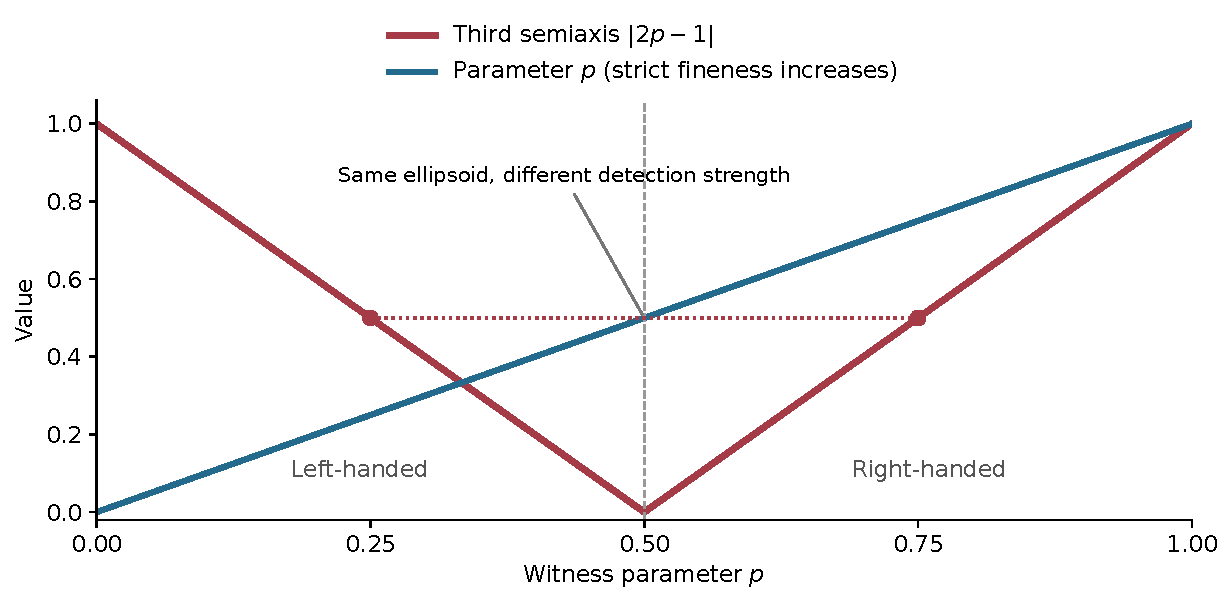
\includegraphics[width=.92\linewidth]{figures/parameter_orders.pdf}
\caption{The two orders for $W_p$. Fineness increases with $p$ throughout the witness interval. The third semiaxis, $|2p-1|$, decreases to zero and then increases. The mirror parameters $p$ and $1-p$ have identical filled ellipsoids.}
\end{figure}

\section{An exact convex program with a unique rank-one optimizer}

The refinement construction can be converted into a practical optimization problem. Fix the positive trace-preserving map $L$ associated with the target as in \eqref{eq:L}, and define the real-linear map on Hermitian matrices
\[
 M(Q)=(L\otimes\id)(Q^\Gamma).
\]
Although $M$ need not be positive on all bipartite positive operators, it maps every positive product operator to a positive operator. It preserves trace.

\begin{theorem}[Unique trace-minimizing refinement]\label{thm:sdp}
For $W\in\Sstar$, consider
\begin{equation}\label{eq:sdp-primal}
 \alpha_*(W)=\min_Q\tr Q,
 \qquad Q\succeq0,\qquad W-M(Q)\succeq0.
\end{equation}
This semidefinite program is feasible, attains its minimum, and has a unique minimizer $Q_*$. Moreover
\begin{enumerate}[label=(\roman*)]
\item $0<\alpha_*(W)\leq1$;
\item $Q_*=qq^\dagger$ for a nonzero entangled vector $q$;
\item $U_*=M(Q_*)/\alpha_*(W)$ is optimal in $\Sstar$;
\item $W=\alpha_*(W)U_*+P_*$, where $P_*\succeq0$ is singular;
\item $\alpha_*(W)=1$ if and only if $W$ is already optimal in $\Sstar$.
\end{enumerate}
The program has sixteen real variables and two Hermitian $4\times4$ positive semidefinite constraints. No rank constraint is imposed.
\end{theorem}
\begin{proof}
Part~I supplies a feasible $Q$. Trace preservation implies $0\leq\tr Q\leq1$. Thus the feasible set is closed and bounded inside the positive semidefinite cone, hence compact. A minimum exists and cannot be zero: a positive matrix of zero trace is zero, and $Q=0$ would require $W\succeq0$.

Suppose a minimizer has rank at least two. Choose a nonzero product vector $v$ in its range and set
\[
 \tau=(v^\dagger Q^+v)^{-1}>0,\qquad Q'=Q-\tau vv^\dagger\succeq0.
\]
Since $M(vv^\dagger)\succeq0$,
\[
 W-M(Q')=W-M(Q)+\tau M(vv^\dagger)\succeq0.
\]
This is feasible and has strictly smaller trace, a contradiction. Thus every minimizer has rank one. Its vector must be entangled, since a product vector would make both terms in $W=M(Q)+P$ positive. Its image is a witness with the whole target ellipsoid and the required chirality, and is optimal by Theorem~\ref{thm:main}.

If two distinct minimizers existed, their average would also minimize the objective. Two rank-one positive operators of equal trace and equal range are identical. Distinct minimizers therefore have different ranges, and their average has rank two, contradicting the preceding paragraph. This proves uniqueness.

If $P_*\succ0$, decreasing $Q_*$ by a sufficiently small positive scalar factor would keep the residual positive and decrease the objective. Hence $P_*$ is singular. Finally $\tr P_*=1-\alpha_*$; the fineness criterion proves the last equivalence.
\end{proof}

The rank-one and uniqueness argument is more general: it applies whenever the program is feasible for a nonpositive-semidefinite $W$ and a positive trace-preserving qubit map $L$. Geometric containment is a sufficient condition for feasibility furnished by Part~I; it is not a necessary condition. The examples below distinguish these statements.

Uniqueness here concerns the refinement selected by \emph{minimum trace}. It does not say that there is only one optimal witness in $\Sstar$, or only one optimal witness finer than a given $W$. Minimizing $\alpha$ maximizes the trace of the removable positive remainder.

\subsection{Dual certificates and exact arithmetic}

With the real Hilbert--Schmidt pairing on Hermitian matrices,
\[
 M^*(X)=\Gamma_B((L^*\otimes\id)(X)).
\]
The dual program is
\begin{equation}\label{eq:sdp-dual}
 \sup_X-\tr(XW),\qquad X\succeq0,\qquad I_4+M^*(X)\succeq0.
\end{equation}
Its sign can be checked without convention-dependent duality rules. For feasible $Q,X$,
\begin{equation}\label{eq:duality-gap}
 \tr Q+\tr(XW)
 =\tr((I+M^*(X))Q)+\tr(X(W-M(Q)))\geq0.
\end{equation}
Thus matching primal and dual values certify exact optimality. Since $M$ preserves trace, $M^*(I)=I$, and $X=\varepsilon I$, $\varepsilon>0$, is strictly dual feasible. Standard semidefinite duality gives zero duality gap \cite{boyd}. This does not by itself assert dual attainment on every boundary instance; primal attainment was proved separately by compactness.

The package includes a numerical solver and exact rational primal--dual examples. Numerical eigenvalue tolerances are reported as diagnostics, not as proofs. For rational examples the independent SymPy verifier checks the residuals and objectives exactly. For arbitrary real-algebraic input, real closed field quantifier elimination gives an exact finite procedure in principle; no practical complexity or numerical conditioning guarantee is claimed.

\subsection{A distinct affine SDP for containment itself}

The exact positive lift and two-qubit decomposability also give a finite convex test for containment. With $L$ fixed by the target and $\|b_W\|<1$,
\begin{equation}\label{eq:containment-sdp}
 \boxed{\E(W)\subseteq\E_*
 \iff \exists P,Q\succeq0:\quad
 W=(L\otimes\id)(P+Q^\Gamma).}
\end{equation}
The forward implication lifts $W$ to a block-positive $V$ and decomposes it. Conversely, $P+Q^\Gamma$ is block positive, has the same Bob marginal as $W$, and its conditional Alice vectors are in the unit ball. Applying $L$ sends them into $\E_*$. Trace preservation also implies $\tr P+\tr Q=1$.

This is an affine semidefinite feasibility problem with two positive $4\times4$ auxiliary matrices, so the containment region is a spectrahedral shadow. It works for singular targets: the linear equality automatically enforces their support restrictions. It uses the two-qubit decomposability theorem, whereas the smaller S-lemma certificate uses a quadratic constraint and one scalar multiplier.

The placement of the positive remainder is different in the two programs:
\begin{center}
\begin{tabularx}{\linewidth}{@{}l X@{}}
\toprule
Question & Exact constraint\\
\midrule
Containment & $W=(L\otimes\id)(P)+M(Q)$, with $P,Q\succeq0$.\\
Refinement & $W=R+M(Q)$, with $R,Q\succeq0$.\\
\bottomrule
\end{tabularx}
\end{center}
For Class D, $(L\otimes\id)(P)$ can be a witness. For example, with target $\operatorname{diag}(1,1,1/2)$ and $W=W_{1/4}$, the containment certificate is $P=\proj{\psi^+}$, $Q=0$, while the optimal refinement certificate is $Q=\proj{\phi^+}/3$, $R=2\proj{\psi^+}/3$.

For a rank-two target, choose $L\circ\mathsf T=L$. Then $(L\otimes\id)(P)=M(P^{\mathsf T})$, so \eqref{eq:containment-sdp} simplifies further:
\[
 \E(W)\subseteq\E_*
 \iff W=M(Q)\ \text{for some }Q\succeq0,\ \tr Q=1,
\]
under the same positive-definite Bob marginal hypothesis. Thus the normalized planar containment region, including positive operators, is the image of the density-matrix set, restricted to positive definite Bob marginals. Taking its closure adds the corresponding product-state limits. This strengthens the planar argument without using an inverse of the singular shape matrix.

\section{Sharp comparison of diagonal Class D mirrors}

Consider
\[
 W_\pm=\tfrac14(\II+a\XX+b\YY\pm c\ZZ),
 \quad 1\geq a\geq b\geq c>0,\quad a+b>1+c.
\]
Both are Class D and share semiaxes $(a,b,c)$. Set
\[
 d=a+b-1>c,\qquad t=1-a+b\geq d,
 \qquad \alpha_-=\frac{d-c}{d+c},\quad\alpha_+=\frac{t-c}{t+c}.
\]

\begin{theorem}[The complete feasible scalar interval]\label{thm:sharp-mirror}
For every real $\alpha$,
\begin{equation}\label{eq:sharp-interval}
 W_--\alpha W_+\succeq0
 \quad\Longleftrightarrow\quad
 \alpha_-\leq\alpha\leq\alpha_+.
\end{equation}
This interval is contained in $(0,1)$, and its width is
\[
 \alpha_+-\alpha_-=\frac{4c(1-a)}{(t+c)(d+c)}.
\]
If $a<1$, every interior coefficient gives a positive definite remainder.
\end{theorem}
\begin{proof}
Use the Bell basis $(\phi^+,\phi^-,\psi^+,\psi^-)$. The $\psi^-$ eigenvalue of the difference forces $\alpha\geq\alpha_-$, while its $\phi^-$ eigenvalue forces $\alpha\leq\alpha_+$. On that interval, the $\phi^+$ eigenvalue exceeds the $\phi^-$ eigenvalue by $(a-b)(1-\alpha)/2\geq0$. The $\psi^+$ eigenvalue is $[(1+a+b)(1-\alpha)+c(1+\alpha)]/4>0$. These are all four eigenvalues. The width follows by common denominators. When the interval has nonzero width and both bounds are strict, all four eigenvalues are positive.
\end{proof}

For the target map with Bloch matrix $\operatorname{diag}(a,b,c)$, the solution of \eqref{eq:sdp-primal} for $W_-$ is exactly
\[
 Q_*=\alpha_-\proj{\phi^+},\qquad U_*=W_+.
\]
An exact dual certificate is $X_*=4\proj{\psi^-}/(d+c)$. The eigenvalues of $I+M^*(X_*)$, in Bell order, are
\[
 0,\quad \frac{2(a+b)}{d+c},\quad \frac{2(b+c)}{d+c},\quad \frac{2(a+c)}{d+c}.
\]
They are nonnegative and $-\tr(X_*W_-)=\alpha_-$. This proves global SDP optimality, not merely the scalar comparison of a fixed pair.

A uniform detection separator for this entire family is
\[
 \rho=\frac{1+a+b}{2(a+b)}\proj{\psi^-}
       +\frac{a+b-1}{2(a+b)}\proj{\psi^+}.
\]
Its expectations are $\tr(\rho W_-)=c/4$ and $\tr(\rho W_+)=-c/4$.

For the original family and an outer canonical representative $W_q$, where $1/2\leq q\leq1$ and $0<p\leq q$, the corresponding exact certificates simplify to
\[
 Q_*=(p/q)\proj{\phi^+},\qquad X_*=(2/q)\proj{\psi^-},\qquad\alpha_*=p/q.
\]
This remains feasible for $p<1-q$, even though $\E(W_p)$ is then \emph{not} contained in $\E(W_q)$. Hence feasibility of the refinement SDP is strictly weaker than geometric containment.

\section{Counterexamples form an open set}

\begin{theorem}[A quantitative robustness ball]\label{thm:robust}
Define
\[
 H_-=\tfrac14(\II+\tfrac34\XX+\tfrac34\YY-\tfrac14\ZZ),
 \qquad J(W)=(I\otimes X)W^\Gamma(I\otimes X).
\]
For every Hermitian trace-zero $\Delta$ with $\|\Delta\|_F<1/48$, the matrices
\[
 W=H_-+\Delta,\qquad U=J(W)
\]
are trace-one Class D witnesses, have exactly the same ellipsoid, and satisfy $W-U/2\succ0$. Thus every such $W$ is nonoptimal in the set defined by its own ellipsoid.
\end{theorem}
\begin{proof}
The map $J$ preserves trace, Hermiticity, block positivity and the geometric ellipsoid: partial transpose and a Bob unitary only reparametrize the allowed Bob effects. It is an isometry for the Frobenius norm. At the centre, $J(H_-)=H_+$ and
\[
 \operatorname{spec}(H_--H_+/2)=\{1/32,1/32,1/32,13/32\}.
\]
Every normalized product expectation of $H_-$ is at least $1/16$. Since $\|\Delta\|_{\mathrm{op}}\leq\|\Delta\|_F<1/48$, block positivity persists with a strictly positive margin. The negative eigenvalues of $H_-$ and $H_+$ are $-1/16$ and $-3/16$. Testing their original eigenvectors shows that $W$ and $U$ remain nonpositive-semidefinite. Since $U$ is unitarily equivalent to $W^\Gamma$, the Class D conclusion follows.

Finally,
\[
 \|\Delta-J(\Delta)/2\|_{\mathrm{op}}
 \leq\tfrac32\|\Delta\|_F<1/32.
\]
This is smaller than the least eigenvalue of the original remainder, so $W-U/2$ is positive definite. The fineness criterion gives strict improvement.
\end{proof}

This is an open ball in the fifteen-dimensional real affine space of trace-one Hermitian matrices. The enclosing ellipsoid varies with $\Delta$; the theorem does not claim that one fixed ellipsoid serves the entire ball. Its purpose is to show that the failure is stable under arbitrary sufficiently small matrix perturbations, including nondiagonal ones.

\section{Convexity and arbitrarily close improvements}

\subsection{A second exact containment criterion}

The support function of the target is
\[
 h_*(n)=n\cdot c_*+\sqrt{n^{\mathsf T}Q_*n}.
\]
For trace-one Hermitian Bloch data with $\|b\|<1$,
\begin{equation}\label{eq:support-containment}
 \boxed{\E(W)\subseteq\E_*
 \iff n\cdot a+\|T^{\mathsf T}n-h_*(n)b\|\leq h_*(n)
 \quad\text{for every }n\in S^2.}
\end{equation}
Indeed, containment is equivalent to $n\cdot r_W(u)\leq h_*(n)$ for every $n,u$. Multiply by the strictly positive denominator and maximize the resulting linear function of $u$ over the unit ball. The maximum is the Euclidean norm in \eqref{eq:support-containment}. The argument works for flat targets as well as solid ones.

For each fixed $n$, this is a second-order-cone constraint affine in the original Bloch coefficients. Thus the region of trace-one Hermitian operators with positive definite Bob marginal and ellipsoid inside $\E_*$ is convex. If $\E_*\subseteq\B$, membership already implies block positivity. The nonpositive-semidefinite condition defining witnesses need not itself define a convex set; the following comparable segments are witnesses throughout.

\begin{theorem}[Arbitrarily close improvements]\label{thm:local}
Every nonoptimal member of $\Sstar$ has arbitrarily close feasible strict improvements. If $\chi(W)<0$, those improvements can be chosen to have negative chirality. Therefore the nonempty left-handed sector of $\Sstar$ has no maximal elements, even when comparisons are restricted to that sector.
\end{theorem}
\begin{proof}
Choose an outer optimal refinement $W=\alpha U+P$ with $0<\alpha<1$ and nonzero $P\succeq0$. For $0<t\leq1$, put
\[
 V_t=(1-t)W+tU,\qquad k_t=\alpha+(1-\alpha)t,
 \qquad\beta_t=\alpha/k_t.
\]
Then
\begin{equation}\label{eq:interpolation}
 W=\beta_tV_t+(t/k_t)P.
\end{equation}
This gives strict fineness for every $t>0$. A state detected by $W$ is also detected by $U$, and hence by their mixture; thus $V_t$ is a witness. The conditional Alice vector of $V_t$ is a positive weighted convex combination of the corresponding vectors for $W$ and $U$, so its ellipsoid remains inside $\E_*$. Equivalently, use \eqref{eq:support-containment}.

The family converges to $W$ in every matrix norm. If $\det\Theta_W<0$, continuity preserves that strict sign for all sufficiently small positive $t$. The main theorem excludes negative-chirality optimal witnesses, so the result applies to every member of the left-handed sector.
\end{proof}

This strengthens the earlier same-chirality example into a statement about every left-handed witness in every admissible enclosure. It also identifies local and global relative optimality: a nonoptimal point cannot be protected by restricting attention to a sufficiently small neighbourhood.

There is a stronger geometric version. For a left-handed $W$, apply the mirror lemma at its own ellipsoid, choosing $U$ with $\E(U)=\E(W)$. The same interpolation then satisfies $\E(V_t)\subseteq\E(W)$. For sufficiently small positive $t$, both witnesses are left-handed and strictly comparable. Their ellipsoids cannot be equal by the fixed-chirality orbit-incomparability lemma. Hence
\[
 \E(V_t)\subsetneq\E(W),\qquad D(W)\subsetneq D(V_t),\qquad V_t\longrightarrow W.
\]
Every left-handed witness therefore has arbitrarily close left-handed improvements with a strictly smaller ellipsoid.

\section{The full family of optima and its limiting states}

Fix the canonical right-handed optimal representative $W_*$ in rank three, or the canonical representative in rank two, with $(W_*)_B=I/2$. The complete set of optima is
\begin{equation}\label{eq:all-optima}
 U_G=\frac{2(I\otimes G)W_*(I\otimes G^\dagger)}{\tr(GG^\dagger)},
 \qquad G\in GL(2,\C).
\end{equation}
This follows from the classification and the fixed-ellipsoid filter-orbit theorem.

Two filters give the same normalized witness exactly when they differ by a nonzero complex scalar. To see this, reduce an equality to a filter preserving $W_*$ up to scale. Its action on the Bob marginal makes it a scalar times a unitary. The associated rotation fixes the row space of the correlation matrix, which has dimension at least two. A proper rotation fixing two independent vectors is the identity, so the unitary is only a phase.

Thus the optimum set is a six-real-dimensional manifold parametrized by $PGL(2,\C)\simeq PSL(2,\C)$. One can equivalently specify a positive definite Bob density matrix and a Bob rotation, with three real parameters each. Distinct members are incomparable by fineness.

Formula~\eqref{eq:all-optima} extends continuously to nonzero singular filters. A rank-one filter $G=\ket b\bra v$ gives the product state
\[
 \rho_A(c_*+A u_v)\otimes\proj{\widehat b},\qquad u_v\in S^2.
\]
In rank three, Alice's Bloch vector lies on the surface of the target. In rank two, $A(S^2)=A(\B)$, so the full filled ellipse occurs. These are exactly the added limiting states. The witness optimum set itself is not closed, because singular-filter limits are positive product states.

For a full-dimensional target there is a precise compactification. The map
\[
 [q]\in\C P^3\longmapsto
 (L\otimes\id)((qq^\dagger)^\Gamma/\|q\|^2)
\]
is a smooth embedding, since $L\otimes\id$ is invertible on the real vector space of Hermitian matrices. The entangled rays give the optimal witness orbit; the product-ray quadric $\C P^1\times\C P^1$ gives its complement in the compactification. Here the word ``boundary'' would mean a complement in the closure, not a codimension-one manifold boundary.

The convex hull of the closure is precisely
\[
 \{M(Q):Q\succeq0,\ \tr Q=1\}.
\]
Every such point is a convex combination of at most four pure-source images, by spectral decomposition. This convex hull is not identified with the entire containment set: the refinement formula can also contain a positive remainder.

For rank two, the additional transpose identity in \eqref{eq:containment-sdp} does identify the closed normalized containment region with this convex hull, provided the singular-marginal product limits are included. The full-dimensional case has no such asserted identification.

\subsection{The order structure at one full-dimensional Class D ellipsoid}

Fix a full-dimensional Class D ellipsoid and consider only witnesses representing exactly that ellipsoid. There are two Bob-filter orbits, distinguished by chirality. Each is a copy of $\operatorname{PGL}_2(\C)$, and each is an antichain for strict fineness by Corollary~\ref{cor:sameE}. Every positive-chirality member is relatively optimal in the entire containment set, while every negative-chirality member has a strictly finer positive-chirality representative. Consequently every strict comparison at fixed ellipsoid goes from negative to positive chirality, and every strict chain has at most two distinct witnesses. This does not claim that every positive-chirality representative refines every negative-chirality one.

The two orbit closures are each homeomorphic to $\C P^3$. Their added product-state sets coincide:
\[
 \{\rho_A(r)\otimes\rho_B(n):r\in\partial\E_*,\ n\in S^2\}.
\]
Indeed, the two invertible correlation maps send the input sphere onto the same ellipsoid surface. Each closure consists of its witness orbit and exactly this product set. Opposite-chirality witnesses cannot coincide, so the intersection of the two closures is exactly that common subset, homeomorphic to the Segre quadric. No holomorphic gluing or manifold structure of the union is asserted. This gives both the order structure and a compact topological description of all representatives of one Class D ellipsoid.

There is a useful explicit caution about the chirality correction. Define
\[
 A=\tfrac14(\II+\tfrac34\XX-\tfrac34\YY+\tfrac14\ZZ),
 \qquad B=A^\Gamma=\tfrac14(\II+\tfrac34\XX+\tfrac34\YY+\tfrac14\ZZ).
\]
These are Class D witnesses with the same ellipsoid and opposite chirality, but neither is finer than the other. Their expectations on $\phi^-$ are $-1/16$ and $5/16$, while those on $\psi^-$ are $3/16$ and $-3/16$. The two Bell states therefore certify both failures of detector inclusion. The mirror theorem promises a suitable right-handed representative; the unadjusted partial transpose need not be that representative.

\section{Class C examples and a geometric obstruction within one chirality}

\subsection{Relative optimality need not be global or weak optimality}

For $1/3<r\leq1$, let
\[
 S_r=\tfrac14(\II+r\XX+r\YY+r\ZZ).
\]
Its spectrum is $(1+r)/4$ with multiplicity three and $(1-3r)/4$. Its partial transpose has eigenvalues $(1+3r)/4$ and $(1-r)/4$ with multiplicity three. It is therefore Class C, with positive chirality and target $r\B$. The classification makes it optimal relative to this target. For $r<1$ it is not globally optimal, since
\[
 S_r=rS_1+(1-r)I_4/4.
\]
It is not weakly optimal in the usual unrestricted sense either: its minimum normalized product expectation is $(1-r)/4>0$. Relative optimality imposes no requirement to touch the Bloch sphere when the prescribed enclosure lies strictly inside it.

\subsection{A Class C comparison with incomparable ellipsoids}

Take
\[
 V=S_{1/2},\qquad W=\tfrac12V+\tfrac12\proj{00}.
\]
Their spectra are $(3,3,3,-1)/8$ and $(11,3,3,-1)/16$, and both partial transposes are positive definite. Thus both witnesses are right-handed Class C, with $V$ strictly finer than $W$. Yet
\[
 \E(V)=\tfrac12\B,\qquad
 c_W=(0,0,1/6),\qquad Q_W=\operatorname{diag}(1/12,1/12,4/9).
\]
The point $(0,0,5/6)$ belongs to $\E(W)$ but not $\E(V)$, while $(1/2,0,0)$ belongs to $\E(V)$ but not $\E(W)$. The ellipsoids are incomparable. For the exact separator
\[
 \rho=\tfrac56\proj{\psi^-}+\tfrac16\proj{00},
 \qquad\tr(V\rho)=-1/24,\qquad\tr(W\rho)=1/16.
\]
The volume of $\E(W)$ is $4/9$ of that of $\E(V)$; neither volume nor a fixed chirality turns geometric containment into the general fineness relation.

The Lean development checks the actual noncanonical fractional map for $W$:
\[
 r_W(u)=\left(\frac{u_1}{4+2u_3},\frac{u_2}{4+2u_3},
                  \frac{2+3u_3}{4+2u_3}\right).
\]
This matters because $W$ has nonzero Bob Bloch vector and the simpler canonical affine-map definition cannot be used for it without whitening.

\begin{figure}[H]
\centering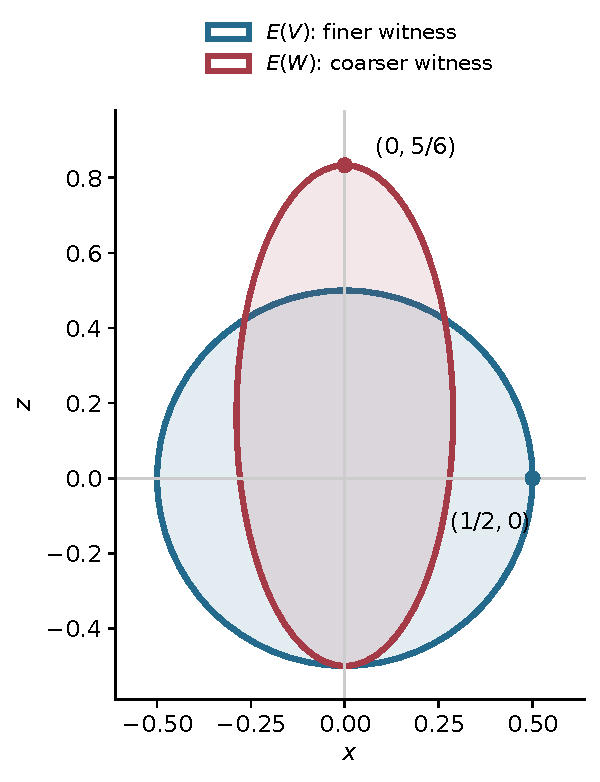
\includegraphics[width=.52\linewidth]{figures/class_c_incomparability.pdf}
\caption{An $xz$ section of the two Class C ellipsoids. The spherical witness $V$ is strictly finer than $W$, but neither ellipse contains the other. The marked points certify both failures of containment.}
\end{figure}

\subsection{Unbounded reversal of ellipsoid volume}

The failure of geometric monotonicity cannot be repaired by replacing containment with volume. For $0<\delta\leq1/8$, define
\[
 V_\delta=\tfrac14[\II+(1-\delta)\XX+\delta\YY+\delta\ZZ],
 \qquad W_\delta=\tfrac34V_\delta+\tfrac14\proj{\phi^-}.
\]
Both are canonical right-handed Class C witnesses. Their positive correlation diagonals are respectively
\[
 (1-\delta,\delta,\delta),\qquad
 \left(\frac{2-3\delta}{4},\frac{1+3\delta}{4},\frac{1+3\delta}{4}\right).
\]
The only negative Bell eigenvalue of $V_\delta$ is $-\delta/4$; that of $W_\delta$ is $-3\delta/16$. Their partial-transpose spectra, in Bell order, are respectively
\[
 \left(\frac{2+\delta}{4},\frac{\delta}{4},\frac{2-3\delta}{4},\frac{\delta}{4}\right),\qquad
 \left(\frac{8+3\delta}{16},\frac{2+3\delta}{16},\frac{4-9\delta}{16},\frac{2+3\delta}{16}\right).
\]
All entries are positive in the stated interval. The state
\[
 \rho=\tfrac78\proj{\psi^-}+\tfrac18\proj{\phi^-}
\]
has expectations $-\delta/8$ and $(1-3\delta)/32$, proving strict fineness of $V_\delta$ over $W_\delta$.

Their volume ratio, with the common ball-volume factor cancelled, is
\[
 \frac{\operatorname{vol}\E(W_\delta)}{\operatorname{vol}\E(V_\delta)}
 =\frac{(2-3\delta)(1+3\delta)^2}{64(1-\delta)\delta^2}
 \longrightarrow\infty\qquad(\delta\downarrow0).
\]
Thus the finer witness can have an arbitrarily smaller ellipsoid, even with positive chirality and Class C fixed. This family is verified algebraically in the accompanying symbolic checks; it is not included among the claimed Lean theorems.



\section{Planar targets, admissibility, and practical decision rules}

For $0<a,b\leq1$ and $a+b>1$, the witness
\[
 D_{a,b}=\tfrac14(\II+a\XX+b\YY)
\]
has a rank-two ellipsoid with semiaxes $a,b,0$. Its Bell eigenvalues are
\[
 (1+a-b)/4,\quad(1-a+b)/4,\quad(1+a+b)/4,\quad(1-a-b)/4.
\]
Its partial transpose is another witness of the same ellipse, so it is Class D. At $a=b=3/4$ this is a radius-$3/4$ disk strictly inside the Bloch ball, with spectrum $\{1/4,1/4,5/8,-1/8\}$. Every witness representing the whole disk is relatively optimal. This supplies a concrete strictly interior planar instance of the singular-target proof.

For any proposed target $c_*+A\B\subseteq\B$ of rank at least two, choose the orientation convention used in Part~I and form
\[
 W_*=(L\otimes\id)(\Phi^\Gamma).
\]
The target is admissible exactly when $W_*$ fails to be positive semidefinite. In full rank, an admissible target is Class C when $W_*^\Gamma\succeq0$ and Class D otherwise. In rank two, admissible targets are Class D. This is a finite matrix test, with the initial containment of the target in the Bloch ball checked independently. It avoids treating the word ``admissible'' as a purely pictorial condition.

The resulting workflow is explicit:
\begin{enumerate}
\item Extract the Pauli data $a,b,T$ and certify witness validity.
\item Check target admissibility and rank. If the rank is at most one, there are no witnesses in its containment set.
\item Certify containment using the support constraints and the S-lemma matrix, or the support-function condition.
\item Test the polynomial equalities and determinant sign in \eqref{eq:polynomial-optimality}.
\item If the witness is not optimal, solve \eqref{eq:sdp-primal}. The exact optimizer has rank one; numerical rank is only a diagnostic.
\item Certify the resulting positive remainder. When available, a matching dual certificate proves minimum trace exactly.
\end{enumerate}

The mathematical existence proof and the implementation serve different purposes. The proof handles singular and exceptional cases exactly. The numerical solver makes examples accessible and can suggest rational certificates, but its floating-point output is never substituted for the mathematical or Lean proofs.

\clearpage
\part{Context, disclosure and verification}
\section{Related work and novelty}\label{sec:related}

The bounded search through 3 November 2026 did not locate a prior resolution of this conjecture. Section~IV\,D of \cite{milne} and Milne's thesis \cite{thesis} are the primary statements. The search covered the works citing \cite{milne} indexed by OpenAlex; this is evidence about a bounded search, not a proof of priority.

Closely related earlier work limits any novelty claim. Best separable approximation, pure two-qubit entangled remainders and uniqueness of separable approximations were developed by Lewenstein--Sanpera and Karnas--Lewenstein \cite{ls,karnas}. Bru\ss{} and coauthors gave a general framework for best positive-part witness decompositions and a unique maximal subtraction \emph{coefficient}, distinguishing uniqueness of the coefficient from uniqueness of the decomposition \cite{bruss}. Their support-of-marginals observation also covers the basic marginal-support phenomenon used here. Semidefinite programming and duality for optimal Lewenstein--Sanpera decompositions were developed by Thiang--Raynal--Englert \cite{thiang}. Optimality of decomposable witnesses and completely entangled subspaces were studied by Augusiak, Tura and Lewenstein \cite{augusiak}.

Accordingly, this paper does not claim to originate positive subtraction, the product-vector removal method, best-decomposition optimization or SDP duality. The candidate contribution is the chirality-sensitive resolution for an arbitrary admissible ellipsoid target, with its target-map formulations and geometric consequences. The unique-source result for \eqref{eq:sdp-primal} is proved here for this explicitly defined positive-map problem; its novelty has not been established by the search.

Several distinctions should survive any later presentation:
\begin{itemize}
\item The literal necessity conjecture and the stronger characterization have different outcomes.
\item Class~C complete positivity cannot be used in Class~D without the mirror comparison.
\item A three-dimensional normal-form proof must include the extraordinary boundary case.
\item A flat target needs support equations and a genuine singular lift.
\item A complete formal counterexample is not a complete formal proof of the corrected classification.
\item Neither relative optimality nor fineness imposes a general monotone ellipsoid-volume order.
\end{itemize}

\section{Research process and AI disclosure}

This is fully autonomous agentic research. Autonomous AI research agents produced the conjecture analysis, the proofs, the Lean development, the exact and numerical verification scripts, the figures and the draft report from which this paper is derived, in an earlier session whose records do not name the system used. Internal AI-assisted reviews in that session, by separate research threads of the same workflow, found no substantive gap in the analytic chain under its stated published inputs; they are not external peer review and are not included.

Opus 5.5 by Anthropic used with Claude Code assessed the upload for this release. It checked the conjecture statement against arXiv:1407.8440v1 and v2, read the central proofs (the fineness criterion, the orbit incomparability lemma, the mirror comparison, the positive lift and the refinement argument) critically, reran the exact scripts and the numerical demonstration, replayed the Lean development from source against the pinned Mathlib with a new whole-project axiom audit, revised the text into this paper and integrated the package into the repository. The mathematics was not changed.

Dev D. Goyal is responsible for publication. The work has not been externally peer reviewed and no expert validation is claimed. The formal scope and its limits are stated in Appendix~\ref{app:formal} and in the package files \texttt{FORMALIZATION\_STATUS.md} and \texttt{VERIFICATION.md}.

\appendix
\section{What the Lean development proves}\label{app:formal}

The formal development uses Lean 4.19.0 and Mathlib at commit
\begin{center}\small\texttt{c44e0c8ee63ca166450922a373c7409c5d26b00b}.\end{center}
It is essential to distinguish its complete formal refutation of the unrestricted converse from the general corrected classification, which is not an end-to-end Lean theorem.

\subsection{The formal mathematical objects}

The matrix modules use genuine complex $4\times4$ matrices in the computational basis $00,01,10,11$, with the usual definitions:
\begin{align*}
 \operatorname{quad}(A,z)&=\operatorname{Re}\sum_{i,j}\overline{z_i}A_{ij}z_j,\\
 \operatorname{PSD}(A)&\iff A=A^\dagger\ \text{and}\ \operatorname{quad}(A,z)\geq0\ \text{for every }z\in\C^4,\\
 \operatorname{State}(\rho)&\iff\operatorname{PSD}(\rho)\ \text{and}\ \tr\rho=1.
\end{align*}
Block positivity quantifies over every pair of complex two-vectors. A witness is Hermitian, has trace one, is block positive and has a negative quadratic-form value. Detection uses $\operatorname{Re}\tr(W\rho)<0$, and fineness quantifies over every complex density matrix. No restriction to real or Bell-diagonal states is hidden in these definitions.

The canonical ellipsoid is the image of the full real unit ball under the affine map read from the matrix's Pauli coefficients; this is the ellipsoid of \cite{milne} for an operator whose Bob marginal is maximally mixed, and canonicality is proved for each example from its actual coefficients. The Class~C comparison uses the full fractional Bloch map and proves positivity of its denominator on the ball; its noncanonical witness is not passed through the canonical definition. The surrounding set in the theorem \texttt{counterexample} is restricted to canonical witnesses, but the companion theorems \texttt{not\_optimal\_in\_any\_containing\_set} and \texttt{parametric\_not\_optimal\_in\_any\_containing\_set} remove that restriction: no set of complex $4\times4$ matrices that contains the finer witness makes the coarser one optimal.

\subsection{Module-by-module coverage}

\begin{longtable}{@{}p{.30\linewidth}p{.65\linewidth}@{}}
\toprule
Module & Kernel-checked mathematical content\\
\midrule\endhead
\texttt{EllipsoidCounterexample} & Direct witness and partial-transpose witness proofs, Pauli coefficients, equal ellipsoids, strict detection inclusion and the rational Class~D counterexample $p=1/4,3/4$.\\[4pt]
\texttt{SameChirality} & A strictly finer negative-chirality witness with a properly smaller ellipsoid, including an exact density-matrix separator.\\[4pt]
\texttt{ParametricFamily} & Exact fineness and strict-fineness orders for all valid parameters; complete ellipsoid containment and equality criteria; Class~C/D endpoint classification; unique scalar subtraction coefficient; sharp common separation margin; the counterexample for every $0<p<1/2$; unique optimizer within the explicitly stated one-parameter family.\\[4pt]
\texttt{ClassCComparison} & Both Class~C witness properties, positive partial transposes, positive subtraction, strict fineness for arbitrary density matrices, actual noncanonical Bloch data, positive denominators, and two points proving incomparable ellipsoids.\\[4pt]
\texttt{NormalFormCertificates} & A Bell-basis PSD equivalence for complex matrices, exact positive remainders for the ordinary and extraordinary Lorentz forms, their coefficient bounds, and the interior example's coercive quadratic identity.\\[4pt]
\texttt{MirrorComparison} & The complete sharp three-parameter comparison interval, its exact width, nonemptiness, and the minimum-coefficient PSD certificate.\\[4pt]
\texttt{GeometryCertificates} & The homogeneous $4\times4$ raw LMI expansion and containment implication; canonical specialization; positive denominators from the strict marginal bound; singular support equations; an explicit failure of metric-only planar containment; diagonal ellipsoid containment, zero axes allowed.\\[4pt]
\texttt{ProductVector} & Determinant zero if and only if tensor-product factorization for a complex four-vector; a determinant-pencil quadratic root; every complex subspace of $\C^2\otimes\C^2$ of dimension at least two contains a nonzero product vector.\\[4pt]
\texttt{OptimalityReduction} & A cofinal-antichain classification theorem, its connection to the actual matrix detection relation, a counted finite rank-reduction argument with a three-step bound, and the exact interpolation identity. The structural matrix hypotheses are explicit inputs.\\
\bottomrule
\end{longtable}

Some entries are unconditional concrete-matrix or geometric theorems; others are explicitly conditional assembly results. Their type signatures, not their file names, determine what has been proved. The files \texttt{THEOREM\_INDEX.md} and \texttt{FORMALIZATION\_STATUS.md} of the package map each statement to its declaration and list the remaining bridges.

\subsection{The decisive formal conclusion}

The theorem \texttt{infinite\_ClassD\_counterexamples} applies to every $0<p<1/2$. It certifies both Class~D witness properties, admissibility of the target, equality of the ellipsoids, strict fineness of $W_{1-p}$ over $W_p$, and nonoptimality of $W_p$ in the canonical containment-defined set. The theorem \texttt{parametric\_not\_optimal\_in\_any\_containing\_set} shows that no set containing $W_{1-p}$ makes $W_p$ optimal. Together they formally refute the characterization reading of the conjecture. They do not bear on the necessity reading, which Theorem~\ref{thm:main} proves conventionally.

\section{What is not an end-to-end Lean proof}\label{app:gaps}

\textbf{Theorem~\ref{thm:main} is a conventional theorem with published inputs, not an unconditional Lean theorem over arbitrary two-qubit matrices.} The following dependencies remain outside the checked matrix chain:

\begin{enumerate}
\item The two-qubit decomposability theorem $\BP=\PSD+\PSD^\Gamma$ \cite{woronowicz}. It is cited, not introduced as a Lean axiom.
\item Existence and completeness of the Lorentz normal forms, including the extraordinary boundary case \cite{avron}. The PSD certificates \emph{inside} both forms are checked; the reduction of every witness to those forms is not.
\item The general Bob-marginal, whitening, local-filter and orbit-incomparability arguments. The abstract cofinal-antichain theorem does not supply them.
\item The exact positive lift for arbitrary translated or singular targets, its Pauli-map interpretation, and the rank-drop formula involving $Q^+$. Product-vector existence is checked separately; the whole PSD subtraction step is not.
\item Necessity in the S-lemma characterization and the general identification of the pseudoinverse metric enclosure with a matrix-defined ellipsoid. Lean proves soundness of the displayed certificate and the exact diagonal case.
\item The general SDP existence and rank-one uniqueness, the robustness ball, the compactification and the volume reversal, which are conventional results with exact symbolic checks where indicated.
\end{enumerate}

The formal assembly theorem \texttt{quantum\_classification\_given\_structural\_inputs} takes three substantive hypotheses besides membership: every feasible witness has a candidate refinement, candidates are mutually incomparable, and normalized witnesses with the same detection set are equal. Given those inputs it proves the final optimality equivalence for the actual detector definitions. Part~I proves the inputs conventionally; the Lean development does not instantiate them for arbitrary admissible ellipsoids. Likewise the counted rank-reduction theorem assumes a positive-remainder rank drop for every source of rank at least two and then proves termination and the step bound.

The sources contain no \texttt{sorry}, \texttt{admit}, added axiom or native evaluation. A whole-project audit, run with the build, enumerates every declaration defined in the nine content modules and requires each declaration other than the Lean~4.19 code-generation auxiliaries to depend only on \texttt{propext}, \texttt{Classical.choice} and \texttt{Quot.sound}.

\section{How to reproduce the work}

\subsection{Lean}

From the package directory \texttt{lean/}, with the Lean version manager \texttt{elan} and network access for the pinned dependencies:
\begin{Verbatim}[fontsize=\small]
lake exe cache get
lake build Main ProjectAxiomAudit
python3 ../scripts/check_axiom_audit.py --log build.log --project .
lake env lean AxiomAudit.lean
\end{Verbatim}
Here \texttt{build.log} is the saved output of the build command. The last command prints the dependency closures and type signatures of 44 selected theorems.

\subsection{Exact algebra and numerical examples}

From the package directory, with SymPy~1.14.0:
\begin{Verbatim}[fontsize=\small]
python3 scripts/run_exact_checks.py
python3 verification/solve_refinement.py --output sdp.json
python3 verification/make_figures.py
\end{Verbatim}
The first command runs the four exact scripts in a temporary copy, which check 159 symbolic identities, the normal-form formulas, five primal--dual pairs and two containment certificates (positivity by all principal minors), and compares each regenerated report byte for byte with the committed one. The SDP script uses floating-point conic optimization (CVXPY) and labels its results as diagnostics. Its sample cases include full-dimensional Class~C, boundary and strictly interior Class~D, a planar target, a translated target, and a case with feasible refinement but failed containment. The five exactly certified optima are $1/3$, $1/3$, $2/5$, $1/4$ and $2/15$. The translated example is a numerical illustration, not an exact certificate. The figures are generated from exact formulas.


\clearpage
\begin{thebibliography}{99}
\bibitem{milne} A. Milne, D. Jennings, and T. Rudolph, \emph{Geometric representation of two-qubit entanglement witnesses}, Physical Review A \textbf{92}, 012311 (2015). \href{https://arxiv.org/abs/1407.8440}{arXiv:1407.8440}; \href{https://doi.org/10.1103/PhysRevA.92.012311}{doi:10.1103/PhysRevA.92.012311}. In particular Sections II, IV\,C and IV\,D.
\bibitem{lewenstein} M. Lewenstein, B. Kraus, J. I. Cirac, and P. Horodecki, \emph{Optimization of entanglement witnesses}, Physical Review A \textbf{62}, 052310 (2000). \href{https://arxiv.org/abs/quant-ph/0005014}{arXiv:quant-ph/0005014}.
\bibitem{woronowicz} S. L. Woronowicz, \emph{Positive maps of low dimensional matrix algebras}, Reports on Mathematical Physics \textbf{10}, 165--183 (1976). \href{https://doi.org/10.1016/0034-4877(76)90038-0}{doi:10.1016/0034-4877(76)90038-0}.
\bibitem{avron} J. E. Avron and O. Kenneth, \emph{Entanglement and the geometry of two qubits}, Annals of Physics \textbf{324}, 470--496 (2009). \href{https://doi.org/10.1016/j.aop.2008.07.007}{doi:10.1016/j.aop.2008.07.007}. Theorem 8.2, Section 9.4, and Appendix B. \href{https://phsites.technion.ac.il/avron/wp-content/uploads/sites/3/2013/05/Ann_Phys_324_470_2009.pdf}{Author-hosted full text}.
\bibitem{polik} I. P\'olik and T. Terlaky, \emph{A survey of the S-lemma}, SIAM Review \textbf{49}, 371--418 (2007). \href{https://doi.org/10.1137/S003614450444614X}{doi:10.1137/S003614450444614X}; \href{https://optimization-online.org/2004/10/968/}{author preprint record}.
\bibitem{augusiak} R. Augusiak, J. Tura, and M. Lewenstein, \emph{A note on the optimality of decomposable entanglement witnesses and completely entangled subspaces}, Journal of Physics A \textbf{44}, 212001 (2011). \href{https://arxiv.org/abs/1012.3786}{arXiv:1012.3786}.
\bibitem{thesis} A. Milne, \emph{Quantum steering ellipsoids}, doctoral thesis, Imperial College London (issued 2016). Conjecture 7.6, p.~99. \href{https://doi.org/10.25560/44111}{doi:10.25560/44111}.
\bibitem{davalos2019} D. Davalos, M. Ziman, and C. Pineda, \emph{Divisibility of qubit channels and dynamical maps}, Quantum \textbf{3}, 144 (2019), Appendix A. \href{https://arxiv.org/abs/1812.11437}{arXiv:1812.11437}.
\bibitem{davalos2023} D. Davalos and M. Ziman, \emph{Quantum dynamics is not strictly bidivisible}, Physical Review Letters \textbf{130}, 080801 (2023), Theorem 3 and its supplemental proof. \href{https://doi.org/10.1103/PhysRevLett.130.080801}{doi:10.1103/PhysRevLett.130.080801}.
\bibitem{boyd} L. Vandenberghe and S. Boyd, \emph{Semidefinite programming}, SIAM Review \textbf{38}, 49--95 (1996). Theorem 3.1. \href{https://web.stanford.edu/~boyd/papers/pdf/semidef_prog.pdf}{Author-hosted full text}.
\bibitem{ls} M. Lewenstein and A. Sanpera, \emph{Separability and entanglement of composite quantum systems}, Physical Review Letters \textbf{80}, 2261 (1998). \href{https://doi.org/10.1103/PhysRevLett.80.2261}{doi:10.1103/PhysRevLett.80.2261}.
\bibitem{karnas} S. Karnas and M. Lewenstein, \emph{Separable approximations of density matrices of composite quantum systems}, Journal of Physics A \textbf{34} (2001). \href{https://arxiv.org/abs/quant-ph/0011066}{arXiv:quant-ph/0011066}; \href{https://doi.org/10.1088/0305-4470/34/35/318}{doi:10.1088/0305-4470/34/35/318}.
\bibitem{bruss} D. Bru\ss, J. I. Cirac, P. Horodecki, F. Hulpke, B. Kraus, M. Lewenstein, and A. Sanpera, \emph{Reflections upon separability and distillability}, Journal of Modern Optics \textbf{49}, 1399--1418 (2002). Theorem 3, Proposition 6, and the support-of-marginals observation. \href{https://arxiv.org/abs/quant-ph/0110081}{arXiv:quant-ph/0110081}; \href{https://doi.org/10.1080/09500340110105975}{doi:10.1080/09500340110105975}.
\bibitem{thiang} G. C. Thiang, P. Raynal, and B.-G. Englert, \emph{Optimal Lewenstein--Sanpera decomposition of two-qubit states using semidefinite programming}, Physical Review A \textbf{80}, 052313 (2009). \href{https://arxiv.org/abs/0909.4599}{arXiv:0909.4599}; \href{https://doi.org/10.1103/PhysRevA.80.052313}{doi:10.1103/PhysRevA.80.052313}.
\end{thebibliography}
\end{document}

